\section{Gripper model}
In this section the choice of the gripper mounted on the test robot is detailed
and explained. The variance within the dataset of chosen objects to grasp being
so large, the chosen gripper has been chosen in order to be as general as
possible, which is the main reason between most of the planning choices behind
it.

The gripper consists of a mounting flange to quickly mount and
dismount it on the robot's base, a aluminium shaft to let the gripper enter
easily into the objects' bin, and a serie of picking tools attached to the end
of the shaft.

The mounting flange is the one shown in fig.~\ref{fig:mounting-flange}. At one
of its side, it is adapted to fit COMAU Racer999's mounting holes. This makes
the gripper easy to mount also by nonexpert users, as mounting it only requires
screws' tightening without prior alignment. On the other side of the flange,
six mounting holes provide a solid basement for the gripper's shaft. 

\begin{figure}[htbp]
  \centering
  \includegraphics[height=3in]{./Graphics/gripper_flange}
  \caption{CAD model of the mounting flange of the gripper, depicting
  Racer999's standard mounting holes and plug for air feeding. \label{fig:mounting-flange}}
\end{figure}

The shaft is composed of a simple aluminium tube, which is both resistant enough
to hold the picking tools and picked object without damage, and slim enough to
fit the bin from which the objects will be picked. This is necessary as the
base of the robot, being it COMAU Racer999 as in this use case or another,
industrial one, will seldom be able to fit the bin with easiness, and to reach
objects close to the side of the bin itself; this would either reduce a lot the
choice of grasp possibilities, or make the grasping algorithm fail completely,
both of which are undesirable situations.

Finally, at the end of the shaft various tools can be applied. Three
tools have been attached in order for the gripper to be suitable for every
object: the preferred ones are two suckers, connected internally to an air
compressor, which can easily grasp most of the big objects, the only
requirement being their surface to be smooth enough. The two suckers are put
onto opposite sides of the shaft, and occupy almost no space on the device. Two
different sizes are needed because  the bigger one could either put too much
force on an object and damage it (using the same pressure of the smaller one),
or be too big to find a suitable surface on the object to pick, in particular
in the case of non-flat objects; the smaller sucker, in this sense, provides a
lot more options for picking poses, at the expense of worsened stability of
the grasp, especially during object's movement, due to the weaker sucking
strength. On the front side of the shaft, also, a picking plier is applied,
which is needed for the smallest or thin objects, and more in general for
every objects for which suction can't be applied: books, for example, can't be
picked properly with sucker as opening their pages could result in damage;
objects with irregular shape, also, wouldn't feel enough force because of air
losses and thus need to be picked by the closing clamp.

Both the shaft and the flange are internally cave: this lets the air and power
cables to be routed into the inner part of the gripper's body. At the middle of
the flange, this routing is exported to the external side and connections are
present for supplies.

The suckers and the plier are commanded electrically by onboard relays; these
are driven by the robot's firmware. A software has been implemented using
COMAU's proprietary language, \emph{PDL2}, as one of the main processes running on the
robot. using PDL2's APIs, the software implements a simple TCP server, which
listens for commands and toggles the gripper between five possible
configurations: in the first one (reset), the gripper just remains idle and all
the relays are shut off. This is the main state used during robot's
movement. In the three next ones (close), the gripper closes all the relays
in forward direction, making the plier close and the suckers start. The air
compression's strength can been controlled onboard for both the suckers at the
same time, by operating onto the air's closing valve. In the last state (open),
the gripper actively releases its pick, by turning on relays in reverse
direction, thus making the plier open and the suckers blow. This last state  is
necessary, especially for suckers, because if they are left idle the vacuum
created while picking the object will remain active and so the object will not
be released.

Using this gripping system, which model can be seen in fig.~\ref{fig:gripper}
every object in the set has a good number of valid grasp poses, from which the
control algorithm can choose from. Interfacing is also simple from the
programmer's side as the gripper is seen as a TCP server, and this has made it
possible to write a simple library to operate it from within every point of the
program.

\begin{figure}[htbp]
  \centering
  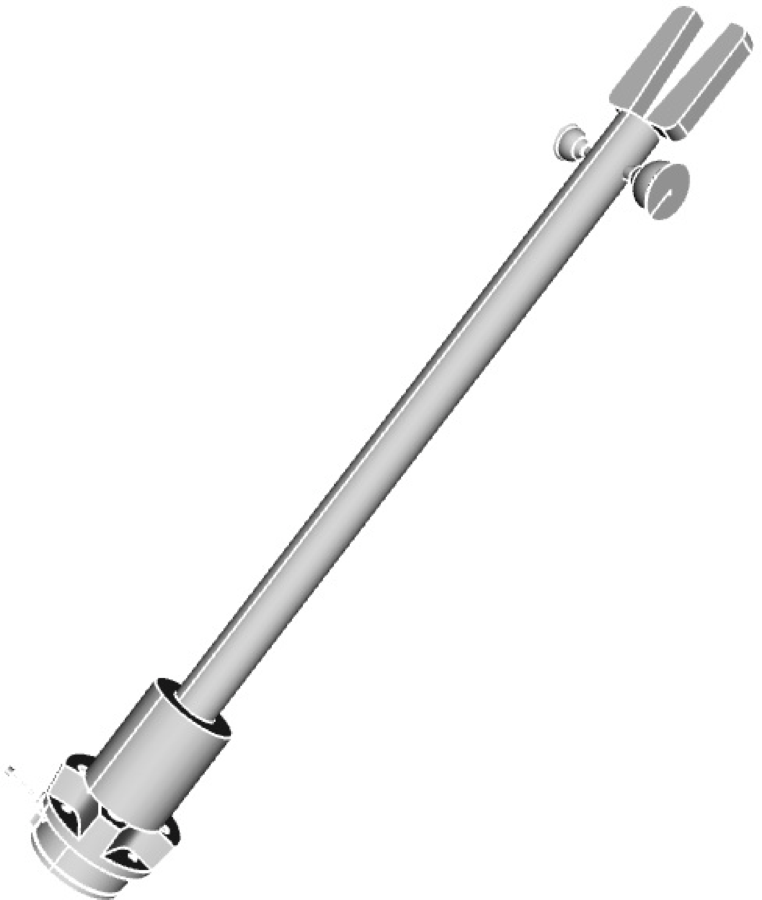
\includegraphics[height=3in]{./Graphics/gripper}
  \caption{CAD model of the gripper, with the two suckers on the sides and
  pliers on the front. \label{fig:gripper}}
\end{figure}

